\documentclass[xcolor=dvipsnames,mathserif]{beamer}
%This is a demo for creating a interactive slide show with latex.
%For fast compile, reduce the the ranges for the for-loops in lines 127, 141, and 142. (This will render less slides and make some buttons inactive.)
%Last update: March 6, 2018
% Created by Alice Schwarze. 


%%%%%%%%%%%%%%%%%%%%%%%%%%%%%%%%%%%%%%%%%%%%%%%%%%

%PACKAGES

%for drawing objects
\usepackage{tikz}

%For adding variables
\usepackage{calc}

%For absolute positioning in beamer
\usepackage[absolute,overlay]{textpos}

%For \ifthenelse
\usepackage{ifthen}

% amsmath and amssymb packages, useful for mathematical formulas and symbols
\usepackage{amsmath,amssymb,mathtools}

%%%%%%%%%%%%%%%%%%%%%%%%%%%%%%%%%%%%%%%%%%%%%%%%%%

%% MACROS

\newcommand\setButtonColor[2]{%
    %This command determines the colour of a tab/ action button. Inactive buttons are blue. Active buttons are magenta.
     \ifnum#1=#2
        magenta%
    \else
         cyan%
    \fi
}

\newcommand\makeSideButton[3]{%
    %This command creates a single button on the right side of the page.
    \node (name) at #2 {\hyperlink{#3-1-0-0}{\tikz\node (name2) [fill=#1,thick, minimum width=2cm, 
                                                                                                minimum height=0.8cm, rotate=90] {#3};}};
}

\newcommand\makeBottomButton[4]{%
    %This command creates a single action button on the bottom of the page.
    \node (name) at #2 {\hyperlink{CrIMs-#3-0-0}{\tikz\node (name2) [fill=#1,thick, minimum width=1.5cm, 
                                                                                                      minimum height=0.7cm] {#4};}};
}

\newcommand\makeSideButtons[1]{%
    %This command creates the tabs/action buttons at the right side of the page.
    \makeSideButton{\setButtonColor{1}{#1}}{(12.4cm, -2.2cm)}{CIMs}
    \makeSideButton{\setButtonColor{2}{#1}}{(12.4cm, -4.7cm)}{CrIMs}
    \makeSideButton{\setButtonColor{3}{#1}}{(12.4cm, -7.2cm)}{EnIMs}
}

\newcommand\makeBottomButtons[1]{%
    %This command creates the tabs/action buttons at the bottom of the page.
    \makeBottomButton{\setButtonColor{1}{#1}}{(1cm, -9.3cm)}{1}{A}
    \makeBottomButton{\setButtonColor{2}{#1}}{(3cm, -9.3cm)}{2}{B}
    \makeBottomButton{\setButtonColor{3}{#1}}{(5cm, -9.3cm)}{3}{C}
    \makeBottomButton{\setButtonColor{4}{#1}}{(7cm, -9.3cm)}{4}{D}
    \makeBottomButton{\setButtonColor{5}{#1}}{(9cm, -9.3cm)}{5}{E}
    \makeBottomButton{\setButtonColor{6}{#1}}{(11cm, -9.3cm)}{6}{F}
}

%These commands specify the offset of the square lattice from the top left corner of the page.
\newcommand\xshift{1.48cm}
\newcommand\yshift{-1.6cm}

\newcommand\makeSquareButton[3]{%
    %This command create a single box that links to another page.
    \node (name) at (\xshift,\yshift) [xshift=#2, yshift=#3]{\hyperlink{#1}{\tikz\node (name2) [xshift=1cm, draw, thick,
                                                                                                                                         minimum width=1cm,
                                                                                                                                         minimum height=1cm] {};}};
}

\newcommand\makeSquareButtons[1]{%
    %This command creates a6x6  lattice of boxes that link to other pages
    \foreach \x in {0,...,5}{%
        \foreach \y in {0,...,5}{%
            \makeSquareButton{CrIMs-#1-\x-\y}{\x cm}{-\y cm}
        }
    }
}

\newcommand\makeTikzOverlay[3]{%
    %This command creates all tabs on the side and bottom of a page and a lattice of boxes to match the heat map.
    \begin{textblock*}{1\textwidth}(0cm,0cm)
        \begin{tikzpicture}[overlay]
            \makeSideButtons{#1}
            \ifthenelse{\equal{#1}{2}}  %if
                           {\makeBottomButtons{#2} %then
                             \makeSquareButtons{#2}}
                           {}%else
        \end{tikzpicture}
    \end{textblock*}
}

\newcommand\makeSquare[2]{%
    %This command makes an orange square that marks the currently selected field in the heat map.
    \begin{textblock*}{1\textwidth}(0cm,0cm)
        \begin{tikzpicture}[overlay]
            \node (name) at (#1cm,-#2cm) [xshift=\xshift, yshift=\yshift, draw=orange, thick, line width=1mm, 
                                                            minimum width=1cm, minimum height=1cm] {};
        \end{tikzpicture}
    \end{textblock*}
}	

%%%%%%%%%%%%%%%%%%%%%%%%%%%%%%%%%%%%%%%%%%%%%%%%%%

\begin{document}

    % First side tab: Covariance-inducing motifs.
    {%Insert plot as local background
    \usebackgroundtemplate{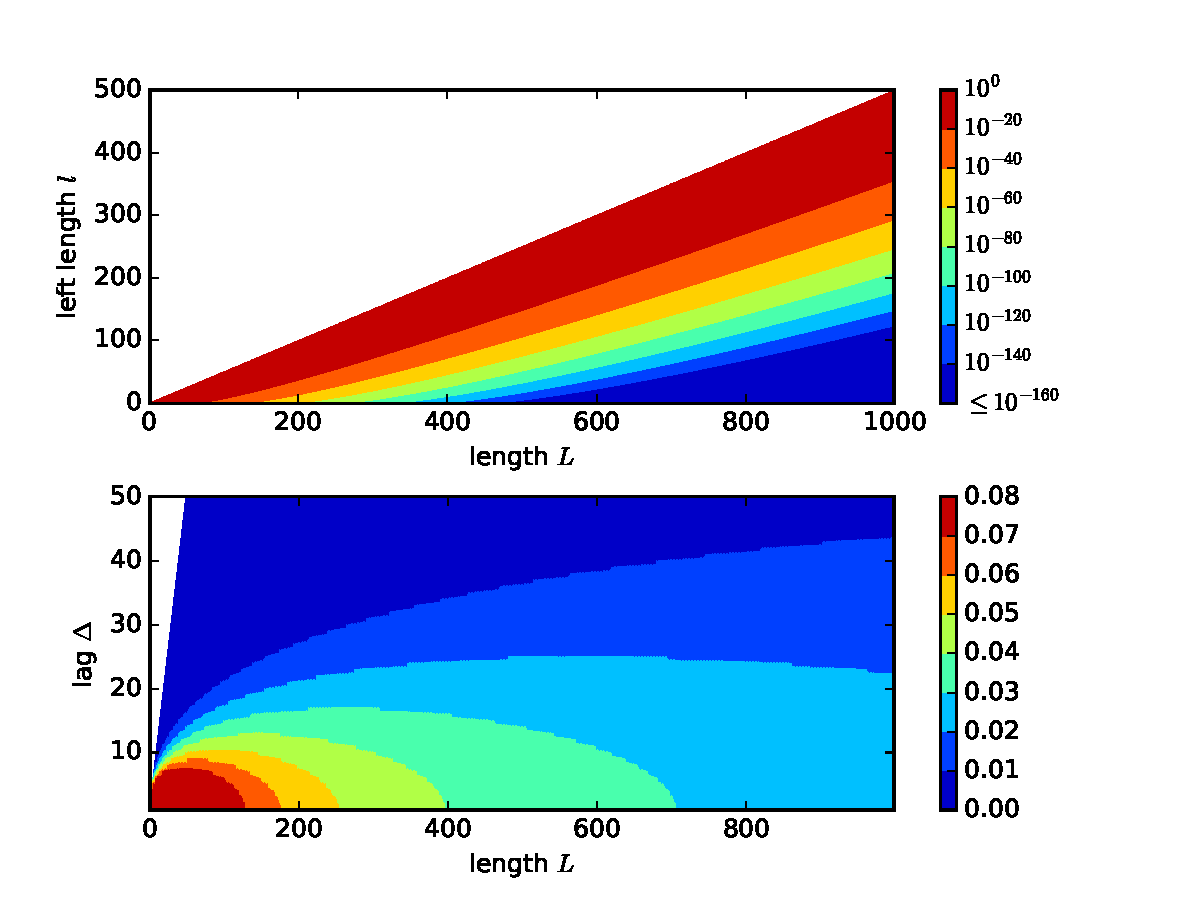
\includegraphics[trim={0cm 0cm 0cm 0cm},clip,height=\paperheight]{plot1}}
        \begin{frame}\label{CIMs-1-0-0}
            \makeTikzOverlay{1}{0}{0} 
            \vspace{3.6cm}\textcolor{white}{
            \begin{equation}
                \hspace{-7cm}\Delta = L-2l
            \end{equation}}
        \end{frame}
    }

    %Third side tab: Entropy-inducing motifs.
    \begin{frame}\label{EnIMs-1-0-0}
        \makeTikzOverlay{3}{0}{0} 
        \begin{center}Work in progress!\end{center}
    \end{frame}

    %Second side tab: Correlation-inducing motifs.
    \newcounter{pagenumber} % Need to count the pagenumbers for motifs.pdf

    \foreach \n in {1,...,6}{%
        %Use for loop to create slides corresponding to the six bottom tabs
        {%Local background
        \usebackgroundtemplate{\includegraphics[trim={0cm 0cm 0cm 1.5cm},clip,height=\paperheight, page=\n]{heatmaps}}
            \foreach \nn in {0,...,5}{%
                \foreach \nnn in {0,...,5}{%
                    % Use two for loops to create slides corresponding to every square in the lattice
                    \setcounter{pagenumber}{36*(\n-1)+6*\nn+\nnn+1}
                    \begin{frame}\label{CrIMs-\n-\nn-\nnn}
                        \makeTikzOverlay{2}{\n}{0} 
                        \makeSquare{\nn}{\nnn}
                        \begin{columns} 
                            \column{0.5\textwidth}
                            \column{0.4\textwidth}
                            \includegraphics[trim={0cm 7cm 21.5cm 3cm},clip,width=4cm,page=\value{pagenumber}]{motifs}
                        \end{columns}
                    \end{frame}
                 }
             }
        }
    }

\end{document}

